\documentclass{standalone}
\usepackage[margin=1in]{geometry}
\usepackage[hang,small,bf]{caption}
\usepackage{tikz}
\usepackage{braket}
\usetikzlibrary{backgrounds,shadows.blur,fit,decorations.pathreplacing,shapes}

\begin{document}
	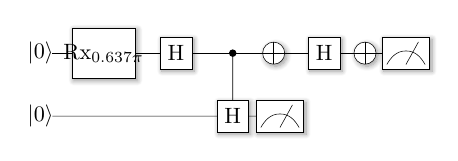
\begin{tikzpicture}[scale=0.8, transform shape]
		
		\tikzstyle{basicshadow}=[blur shadow={shadow blur steps=8, shadow xshift=0.7pt, shadow yshift=-0.7pt, shadow scale=1.02}]\tikzstyle{basic}=[draw,fill=white,basicshadow]
		\tikzstyle{operator}=[basic,minimum size=1.5em]
		\tikzstyle{phase}=[fill=black,shape=circle,minimum size=0.1cm,inner sep=0pt,outer sep=0pt,draw=black]
		\tikzstyle{none}=[inner sep=0pt,outer sep=-.5pt,minimum height=0.5cm+1pt]
		\tikzstyle{measure}=[operator,inner sep=0pt,minimum height=0.5cm, minimum width=0.75cm]
		\tikzstyle{xstyle}=[circle,basic,minimum height=0.35cm,minimum width=0.35cm,inner sep=-1pt,very thin]
		\tikzset{
			shadowed/.style={preaction={transform canvas={shift={(0.5pt,-0.5pt)}}, draw=gray, opacity=0.4}},
		}
		\tikzstyle{swapstyle}=[inner sep=-1pt, outer sep=-1pt, minimum width=0pt]
		\tikzstyle{edgestyle}=[very thin]
		
		\node[none] (line0_gate0) at (0.1,-0) {$\Ket{0}$};
		\node[none] (line0_gate1) at (0.6000000000000001,-0) {};
		\node[none,minimum height=0.8cm,outer sep=0] (line0_gate2) at (1.1,-0) {};
		\node[none] (line0_gate3) at (1.6,-0) {};
		\draw[operator,edgestyle,outer sep=1.0cm] ([yshift=0.4cm]line0_gate1) rectangle ([yshift=-0.4cm]line0_gate3) node[pos=.5] {Rx$_{0.637\pi}$};
		\draw (line0_gate0) edge[edgestyle] (line0_gate1);
		\node[none] (line0_gate4) at (2.0,-0) {};
		\node[none,minimum height=0.5cm,outer sep=0] (line0_gate5) at (2.25,-0) {};
		\node[none] (line0_gate6) at (2.5,-0) {};
		\draw[operator,edgestyle,outer sep=0.5cm] ([yshift=0.25cm]line0_gate4) rectangle ([yshift=-0.25cm]line0_gate6) node[pos=.5] {H};
		\draw (line0_gate3) edge[edgestyle] (line0_gate4);
		\node[none] (line1_gate0) at (0.1,-1) {$\Ket{0}$};
		\node[none] (line1_gate1) at (2.9,-1) {};
		\node[none,minimum height=0.5cm,outer sep=0] (line1_gate2) at (3.15,-1) {};
		\node[none] (line1_gate3) at (3.4,-1) {};
		\draw[operator,edgestyle,outer sep=0.5cm] ([yshift=0.25cm]line1_gate1) rectangle ([yshift=-0.25cm]line1_gate3) node[pos=.5] {H};
		\node[phase] (line0_gate7) at (3.15,-0) {};
		\draw (line0_gate7) edge[edgestyle] (line1_gate2);
		\draw (line1_gate0) edge[edgestyle] (line1_gate1);
		\draw (line0_gate6) edge[edgestyle] (line0_gate7);
		\node[xstyle] (line0_gate8) at (3.8,-0) {};
		\draw[edgestyle] (line0_gate8.north)--(line0_gate8.south);
		\draw[edgestyle] (line0_gate8.west)--(line0_gate8.east);
		\draw (line0_gate7) edge[edgestyle] (line0_gate8);
		\node[none] (line0_gate9) at (4.35,-0) {};
		\node[none,minimum height=0.5cm,outer sep=0] (line0_gate10) at (4.6,-0) {};
		\node[none] (line0_gate11) at (4.85,-0) {};
		\draw[operator,edgestyle,outer sep=0.5cm] ([yshift=0.25cm]line0_gate9) rectangle ([yshift=-0.25cm]line0_gate11) node[pos=.5] {H};
		\draw (line0_gate8) edge[edgestyle] (line0_gate9);
		\node[xstyle] (line0_gate12) at (5.249999999999999,-0) {};
		\draw[edgestyle] (line0_gate12.north)--(line0_gate12.south);
		\draw[edgestyle] (line0_gate12.west)--(line0_gate12.east);
		\draw (line0_gate11) edge[edgestyle] (line0_gate12);
		\node[measure,edgestyle] (line0_gate13) at (5.899999999999999,-0) {};
		\draw[edgestyle] ([yshift=-0.18cm,xshift=0.07500000000000001cm]line0_gate13.west) to [out=60,in=180] ([yshift=0.035cm]line0_gate13.center) to [out=0, in=120] ([yshift=-0.18cm,xshift=-0.07500000000000001cm]line0_gate13.east);
		\draw[edgestyle] ([yshift=-0.18cm]line0_gate13.center) to ([yshift=-0.07500000000000001cm,xshift=-0.18cm]line0_gate13.north east);
		\draw (line0_gate12) edge[edgestyle] (line0_gate13);
		\node[measure,edgestyle] (line1_gate4) at (3.9,-1) {};
		\draw[edgestyle] ([yshift=-0.18cm,xshift=0.07500000000000001cm]line1_gate4.west) to [out=60,in=180] ([yshift=0.035cm]line1_gate4.center) to [out=0, in=120] ([yshift=-0.18cm,xshift=-0.07500000000000001cm]line1_gate4.east);
		\draw[edgestyle] ([yshift=-0.18cm]line1_gate4.center) to ([yshift=-0.07500000000000001cm,xshift=-0.18cm]line1_gate4.north east);
		\draw (line1_gate3) edge[edgestyle] (line1_gate4);
		
	\end{tikzpicture}
\end{document}